\documentclass{article}
\usepackage[utf8]{inputenc}
\usepackage{indentfirst}
\usepackage{titling}
\usepackage{geometry}
\usepackage{graphicx}
\graphicspath{ {./Images/} }
\usepackage[shortlabels]{enumitem}
\usepackage{fancyhdr}
\usepackage{ulem}
\usepackage[dvipsnames]{xcolor}
\usepackage{amssymb}
\usepackage{listings}
\usepackage{color}

\definecolor{dkgreen}{rgb}{0,0.6,0}
\definecolor{gray}{rgb}{0.5,0.5,0.5}
\definecolor{mauve}{rgb}{0.58,0,0.82}

\lstset{frame=tb,
  language=Java,
  aboveskip=3mm,
  belowskip=3mm,
  showstringspaces=false,
  columns=flexible,
  basicstyle={\small\ttfamily},
  numbers=none,
  numberstyle=\tiny\color{gray},
  keywordstyle=\color{blue},
  commentstyle=\color{dkgreen},
  stringstyle=\color{mauve},
  breaklines=true,
  breakatwhitespace=true,
  tabsize=3
}

\def\ojoin{\setbox0=\hbox{$\bowtie$}%
  \rule[-.02ex]{.25em}{.4pt}\llap{\rule[\ht0]{.25em}{.4pt}}}
\def\leftouterjoin{\mathbin{\ojoin\mkern-5.8mu\bowtie}}
\def\rightouterjoin{\mathbin{\bowtie\mkern-5.8mu\ojoin}}
\def\fullouterjoin{\mathbin{\ojoin\mkern-5.8mu\bowtie\mkern-5.8mu\ojoin}}

\renewcommand\maketitlehooka{\null\mbox{}\vfill} %para centralizar verticalmente
\renewcommand\maketitlehookd{\vfill\null}
\pagestyle{fancy}
\fancyhf{}
\rfoot{\thepage}
\lfoot{ 
\includegraphics[scale=0.01]{UA.jpg} José Mendes 107188 LEI}
\geometry{
  a4paper,
  headheight=4cm,
  top=5.5cm,
  bottom=4.5cm,
  footskip=4cm
}


\title{Inteligência Artificial}
\author{José Mendes 107188}
\date{2023/2024}

\begin{document}


\begin{titlepage}
    \maketitle
    \begin{center}
        
\includegraphics[scale=0.4]{UA.png}
    \end{center}
    \thispagestyle{empty} %remove o count da pagina
\end{titlepage}

\pagebreak

\section{Noções de Programação Declarativa}

\subsection{Programação Declarativa}

A Programação Declarativa abstrai-se da implementação, focando-se
apenas na descrição do que se pretende fazer, enquanto faz uso de dois
paradigmas:
\begin{itemize}
  \item \textbf{Programação Funcional}, baseado em funções/calculo-lambda, a entidade central é a função;
  \item \textbf{Programação em Lógica}, baseado em lógica de primeira ordem, a entidade central é o predicado;
\end{itemize}


\subsection{Paradigma Imperativo}

O fluxo de operações é especialmente sequenciado de operações com
foco na forma como as tarefas são executadas (\textbf{instrução}). Podemos \textbf{alterar
o conteúdo em memória} e ainda (instruções de afetação/atribuição) e ainda
\textbf{realizar análise de casos} (if-then-else, switch/case, \dots), \textbf{processamento
iterativo} (while, repeat, for, \dots) e ter associados \textbf{sub-programas} (procedimentos,
funções).

\begin{flushleft}
\textbf{Exemplo:} SQL é uma linguagem declarativa, uma vez que nos seus comandos apenas descrevemos o que queremos obter.
Assim, o programador é abstraído da forma como as operações são executadas na prática, ficando essa tarefa a cargo
do compilador.
\end{flushleft}

\subsection{Paradigma Declarativo}

\begin{center}
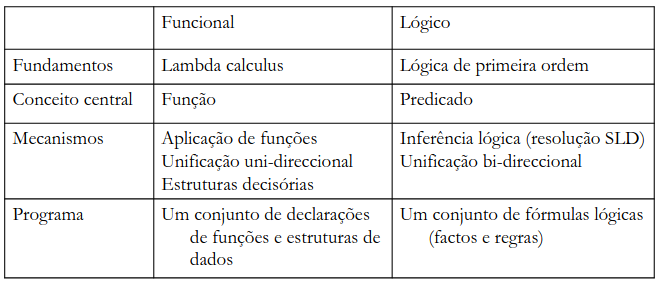
\includegraphics[scale=0.5]{1}
\end{center}

A sua origem data da segunda metade do século XX, mas ainda hoje é amplamente usada e
até está em crescimento em áreas como a Inteligência Artifical.

\pagebreak

\subsection{Programação Funcional}

Possibilidade de definir funções localmente e sem nome. Por exemplo as
funções lambda presentes em Lisp e Python.

\subsection{Programação em Lógica}

Um programa é uma teoria sobre um domínio. Por exemplo, temos
\textbf{socrates é um homem}, $homem(socrates)$ e, um \textbf{homem é mortal}, $homem(X) :- \hspace{1mm} mortal(X)$.
Se perguntarmos se \textbf{socrates é mortal}, $mortal(socrates)$, a resposta é \uline{sim}.

\subsection{Atitude do programador}

A programação declarativa, dada a sua elevada expressividade, é pouco
compatível com aproximações empíricas (ou seja, tentativa e erro) à programação.
Primeiro é preciso pensar bem na estrutura do problema antes de começar a teclar.

\vspace{2mm}

\begin{flushleft}
  \textbf{Passos a seguir:} Perceber o problema $\rightarrow$ Desenhar o programa $\rightarrow$
  Escrevê-lo $\rightarrow$ Rever e testar
\end{flushleft}

\subsection{Características da Programação Funcional}

\begin{itemize}
  \item A entidade central é a função;
  \item A noção de função é diretamete herdada da matemática (ao contrário das
  linguagens imperativas, que pode ser muito diferente);
  \item A estrutura de controlo fundamental é a "aplicação de funções";
  \item A noção de "tipo da função" captura a noção matemática de
  domínio (de entrada e saída);
  \item Os elementos do domínio de entrada e saída podem ser funções;
\end{itemize}

\subsection{Função}

Tem valores de entrada (domínio) e valores de saída (contradomínio).

\begin{center}
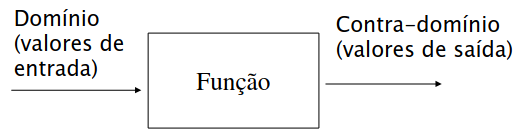
\includegraphics[scale=0.4]{2}
\end{center}

\subsection{Programação em Lógica}

Um programa numa linguagem baseada em lógica representa uma teoria sobre um
problems. Um programa é uma sequência de frases ou fórmulas representando
\textbf{factos} (informação sobre objetos do problema/domínio de aplicação) e \textbf{regras}
(leis gerais sobre esse problema/domínio). Implicitamente as frases estão reunidas
nume grande conjunção, e cada frase está universalmente quantificada. Portanto,
\textbf{programação declarativa}.

\pagebreak

\section{Programação ao estilo funcional em Python}


\end{document}